\chapter{Getting Started}
WEC-Sim is implemented in MATLAB \cite{matlab2014} and running the code requires that you install MATLAB, the MATLAB toolboxes presented in Table~\ref{tab:requiredSoftware}, and the WEC-Sim source code. WEC-Sim was developed in MATLAB R2014a and we recommend using this MATLAB version. In this chapter we describe how to download and install WEC-Sim (Section~\ref{sec:instillation}) and how to run a WEC-Sim simulation (Section~\ref{sec:running}).

\section{Downloading and Installing WEC-Sim} \label{sec:instillation}

\textbf{Step 1: Install MATLAB}\\
Download and install MATLAB and the MATLAB toolboxes presented in Table~\ref{tab:requiredSoftware}. Ensure you have the required toolboxes installed by running the \texttt{ver} command from the \href{http://www.mathworks.com/help/matlab/matlab_env/enter-statements-in-command-window.html}{MATLAB Command Window} (Figure~\ref{fig:installMATLAB}). Consult the MathWorks website \href{http://www.mathworks.com}{http://www.mathworks.com} for more information on performing this step.\\

\begin{table}
\begin{center}
\protect\caption{Required MATLAB toolboxes}\label{fig:installMATLAB}
\begin{tabular}{| l | c |}
\hline
 	\textbf{Matlab package}&\textbf{Required release} \\
\hline
	MATLAB Base&R2014a Version 8.3 \\
\hline
	Simulink&R2014a Version 8.3 \\
\hline
	SimMechanics&R2014a Version 4.4 \\
\hline
	Simscape&R2014a Version 3.11 \\
\hline
\end{tabular}
\label{tab:requiredSoftware}
\end{center}
\end{table}

\begin{figure}[H]
\noindent \begin{centering}
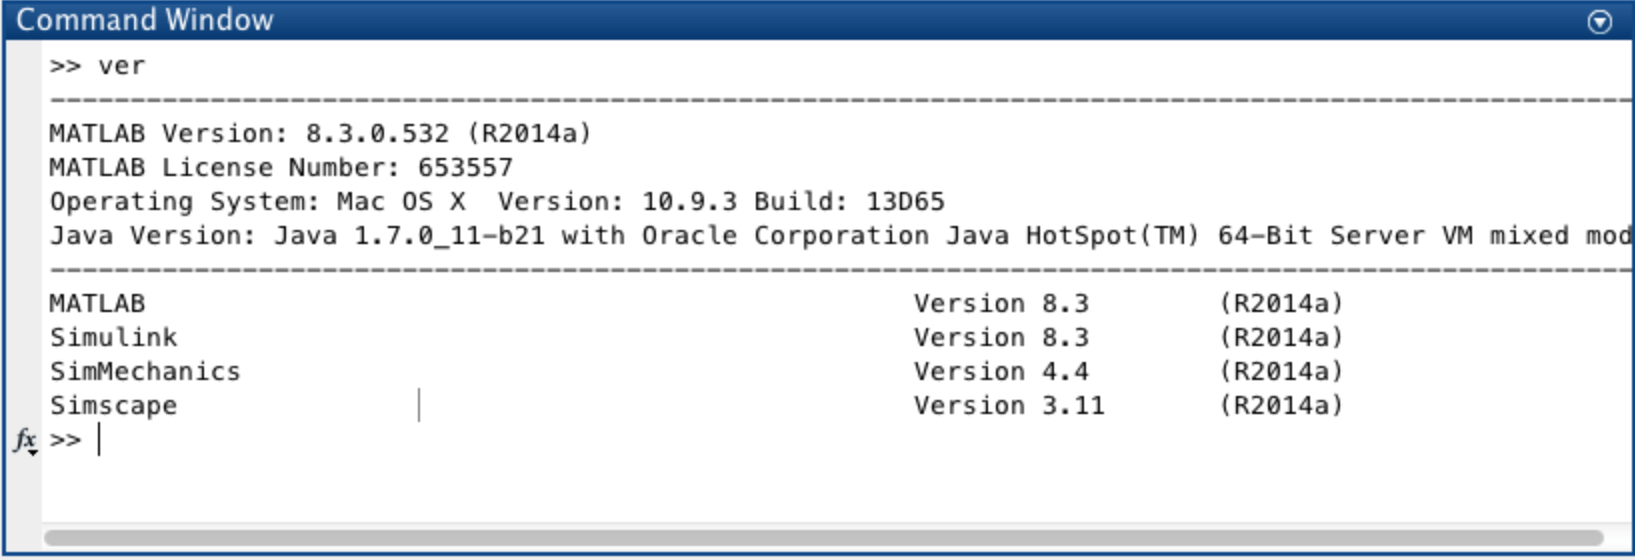
\includegraphics[scale=0.4]{gettingStarted/Figures/installMATLAB}
\protect\caption {Running the \texttt{ver} command from the MATLAB Command Window.}
\par\end{centering}
\end{figure}

\textbf{Step 2: Download WEC-Sim}\\
Download WEC-Sim from the OpenEI website \href{http://en.openei.org/wiki/WEC-Sim/}{http://en.openei.org/wiki/WEC-Sim/}.

\textbf{Step 3: Add the WEC-Sim Source Code to the MATLAB Search Path}\\
Open the \texttt{wecSimStartup.m} file that is located in the \texttt{source} folder within the WEC-Sim source code directory (referred to as \texttt{wecSimSource} in this document). Copy the code in the \texttt{wecSimStartup.m} file and paste it into the \texttt{startup.m} file within the \href{http://www.mathworks.com/help/matlab/matlab_env/matlab-startup-folder.html}{MATLAB Startup Folder}. Set the \texttt{wecSimPath} variable to the location of the \texttt{wecSimSource} folder on your computer. Close MATLAB, restart the code, and then run the \texttt{path} command from the MATLAB Command Window to verify that that the directories listed in \texttt{wecSimStartup.m} are in the \href{http://www.mathworks.com/help/matlab/search-path.html}{MATLAB Search Path}.

\textbf{Step 4: Add the WEC-Sim Blocks to the Simulink Library Browser}\\
Open the Simulink Library Browser by typing \texttt{simulink} from the MATLAB Command Window. Once the Simulink Library Browser opens, select \texttt{View}$\rhd$\texttt{Refresh Tree View}. At this point, you should be able to expand the WEC-Sim menu in the \texttt{Libraries} pane to view the WEC-Sim \texttt{Body}, \texttt{Constraints}, \texttt{PTOs}, and \texttt{Frame} blocks. The function of these blocks will be explained in \hyperlink{chapter.4}{Chapter 4}. From now on, every time you open Simulink in the WEC-Sim Library Browser, the WEC-Sim \texttt{Body Elements}, \texttt{Constraints}, \texttt{PTOs}, and \texttt{Frames} blocks will be available. For more help using and modifying library blocks, please refer to the Simulink Documentation \href{http://www.mathworks.com/help/simulink/}{http://www.mathworks.com/help/simulink/}.

\section{Running WEC-Sim} \label{sec:running}
This section gives an overview of the WEC-Sim work flow and how to run WEC-Sim. Here we describe the file structure of the WEC-Sim runs and the steps for setting up and running a WEC-Sim simulation. Detailed descriptions and options for input parameters for the input file are described in \hyperlink{chapter.5}{Chapter 5}. Specific examples of using WEC-Sim to simulate WEC devices are presented in \hyperlink{chapter.6}{Chapter 6}. 

\subsection{File Structure Overview} \label{sec:fileStructure}
Table \ref{Table: List of default file name and location} shows the default file structure for WEC-Sim. All the necessary files for running WEC-Sim are located within a user defined folder, referred to herein as the WEC-Sim case folder or case directory.

\begin{table}[H]
\noindent \centering{}
\protect\caption{Default files names and their locations}
\begin{tabular}{|c|c|c|}
\hline 
 & \textbf{File name} & \textbf{Location}\tabularnewline
\hline 
Input file & wecSimInputFile.m & Case directory\tabularnewline
\hline 
WEC Model & WEC Model Name.slx & Case directory\tabularnewline
\hline 
WAMIT & WAMIT File Name.out & wamit\tabularnewline
\hline 
Geometry & STL File Name.stl & geometry\tabularnewline
\hline 
\end{tabular}
\label{Table: List of default file name and location}
\end{table}

\subsection{Steps To Run WEC-Sim} \label{sec:stepRunning}
The overview of the WEC-Sim work flow is shown in Figure \ref{fig: WEC-Sim Workflow}. We describe the steps in setting up and running a WEC-Sim simulations in the following:\\

\textbf{Step 1: Pre-Processing}\\
Run WAMIT to generate the hydrodynamic coefficients for each body of the WEC device. WEC-Sim will read the WAMIT-generated hydrodynamic coefficients from the WAMIT output file (\texttt{<wamit file name>.out}). To ensure that WEC-Sim uses the correct hydrodynamic coefficients to model the WEC system, the center of gravity for each body MUST be at the origin of the body coordinate system (XBODY) in WAMIT. Note that the current version of WEC-Sim does not account for the multidirectional wave heading and WEC-Sim will use whatever wave heading was modeled in WAMIT. More details on WAMIT setup are given in the WAMIT User Manual \cite{Lee2006}.

Next the user must create representations of the WEC bodies in the \href{http://en.wikipedia.org/wiki/STL_(file_format)}{STL file format}. The STL files are used to visualize the WEC bodies in the WEC-Sim/MATLAB graphical user interface.\\
 
\begin{figure}[H]
\noindent \centering{}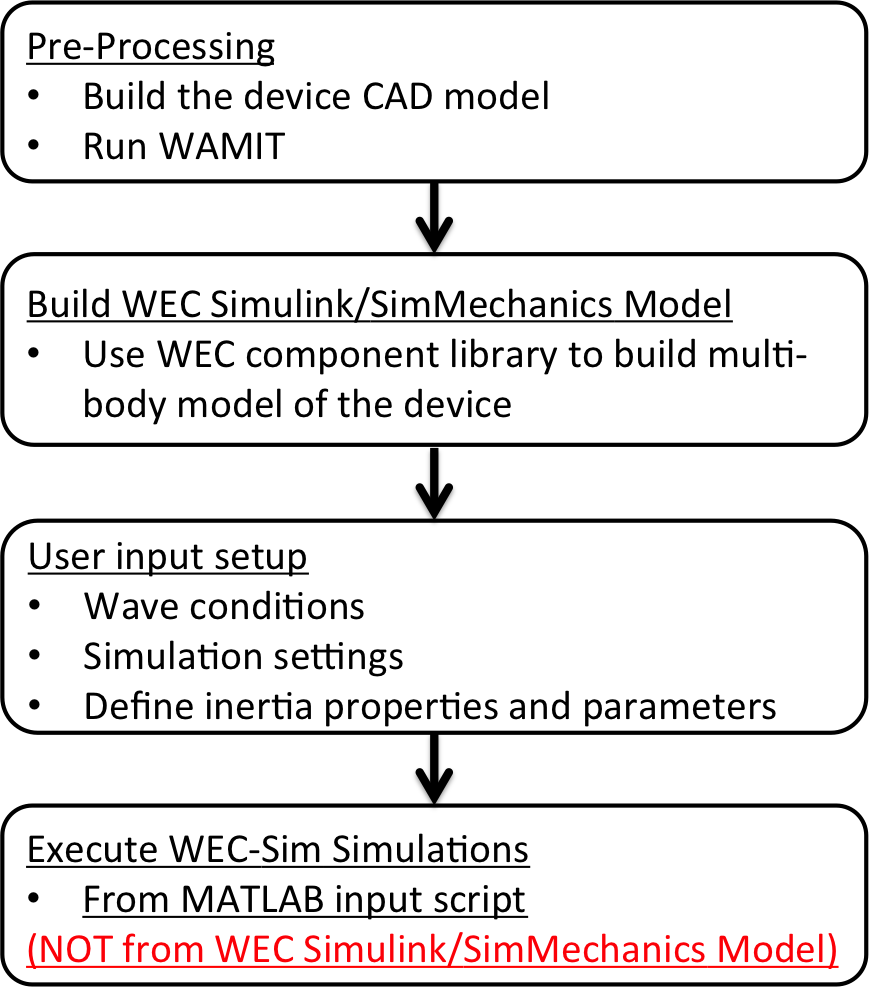
\includegraphics[scale=0.65]{gettingStarted/Figures/WECSimWorkflow}\protect\caption{Work flow diagram for running WEC-Sim simulations}
\label{fig: WEC-Sim Workflow}
\end{figure}

\textbf{Step 2: Build Device Simulink/SimMechanics Model}\\
Next, the user must build the device model using the Simulink/SimMechanics toolboxes and the WEC-Sim Library (see \hyperlink{chapter.4}{Chapter 4}). Figure \ref{fig:wecModel}  shows an example of a a two-body point absorber modeled in Simulink/SimMechanics.

\begin{figure}[H]
\noindent \begin{centering}
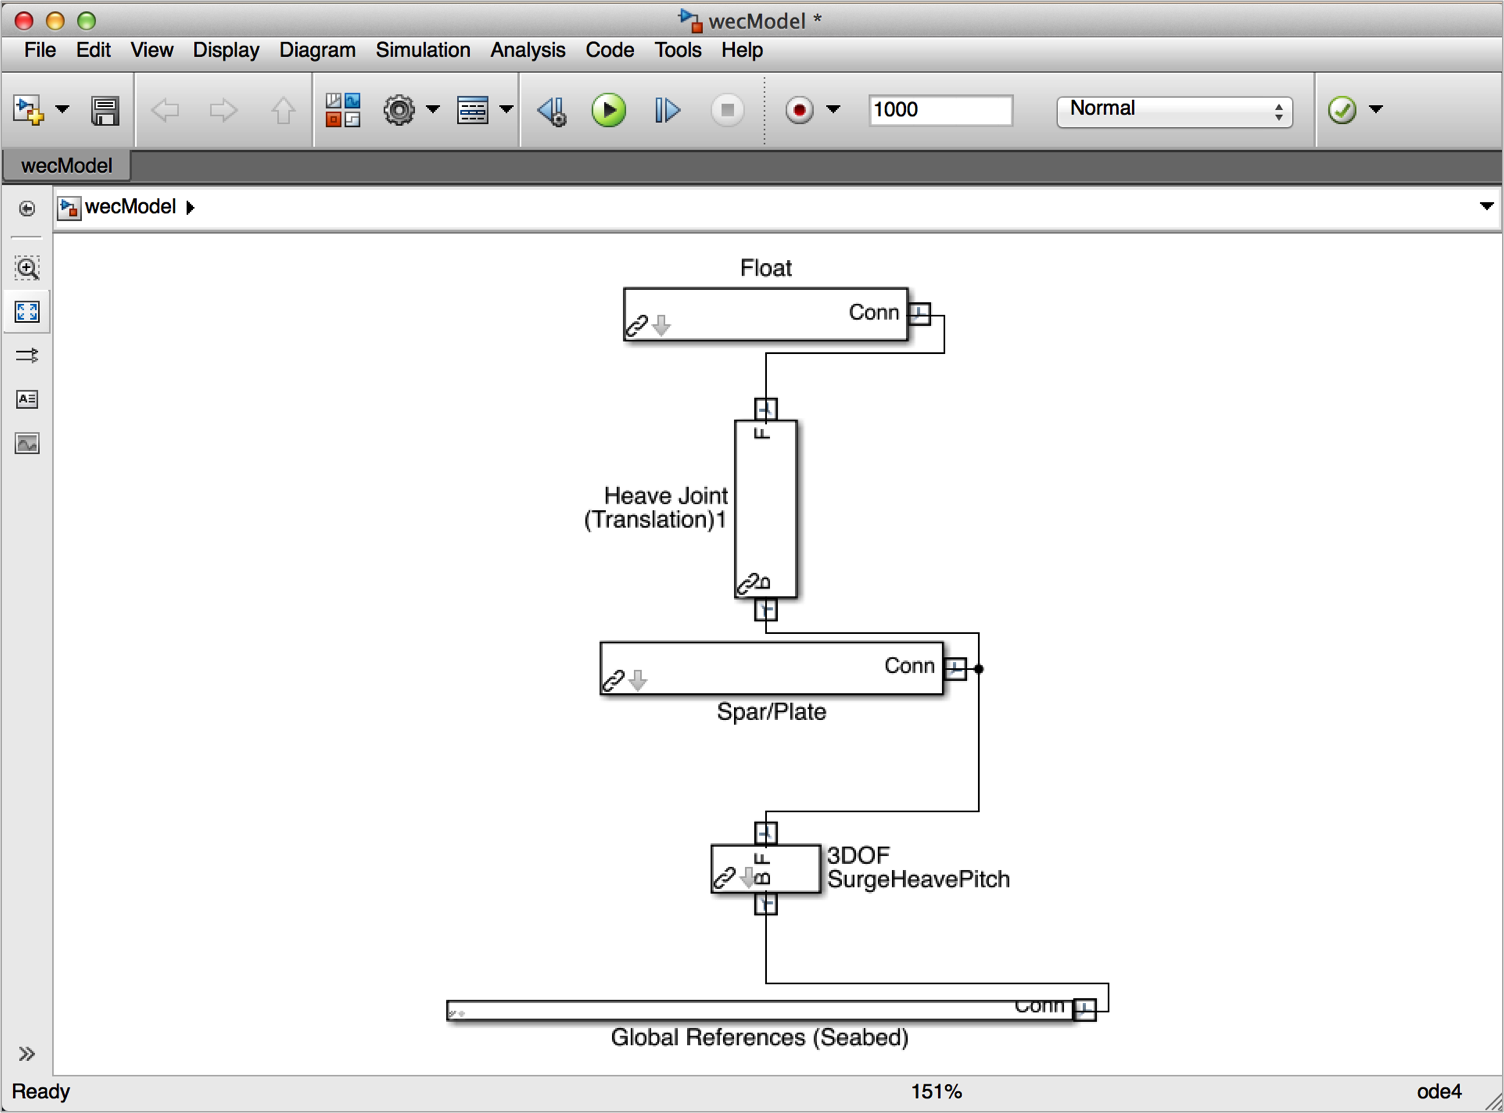
\includegraphics[scale=0.5]{gettingStarted/Figures/exampleWecModel}\protect\caption{An example of device Simulink/SimMechanics model for a two-body point
absorber}
\label{fig:wecModel}
\par\end{centering}
\end{figure}

\textbf{Step 3: Create WEC-Sim Input File}\\
A WEC-Sim input file needs to be created in the case directory, and it MUST be named \texttt{wecSimInputFile.m}. An example of the input file for a two-body point absorber is shown in Figure \ref{fig:exampleRunWECSim}. In the input file, the simulation settings, sea state, body mass properties, PTO, and constraints are specified. In addition, users MUST specify the Simulink/SimMechanics model file name in the \texttt{wecSimInputFile.m}, which is

\begin{center}\texttt{\qquad{}simu.simMechanicsFile='<WEC Model Name>.slx'.}\end{center}

\textbf{Step 4: Execute WEC-Sim}\\
Finally, execute the simulation by running the \texttt{wecSim} command from the MATLAB Command Window (Figure \ref{fig:exampleRunWECSim}). The \texttt{wecSim} command must be executed in the WEC-Sim case directory where the \texttt{wecSimInputFile.m} is located.

WEC-Sim simulations should always be executed from the MATLAB Command Window and not from the Simulink/SimMechanics model. This ensures that the correct variables are in the MATLAB workspace during simulation. 

\begin{figure}[H]
\noindent \centering{}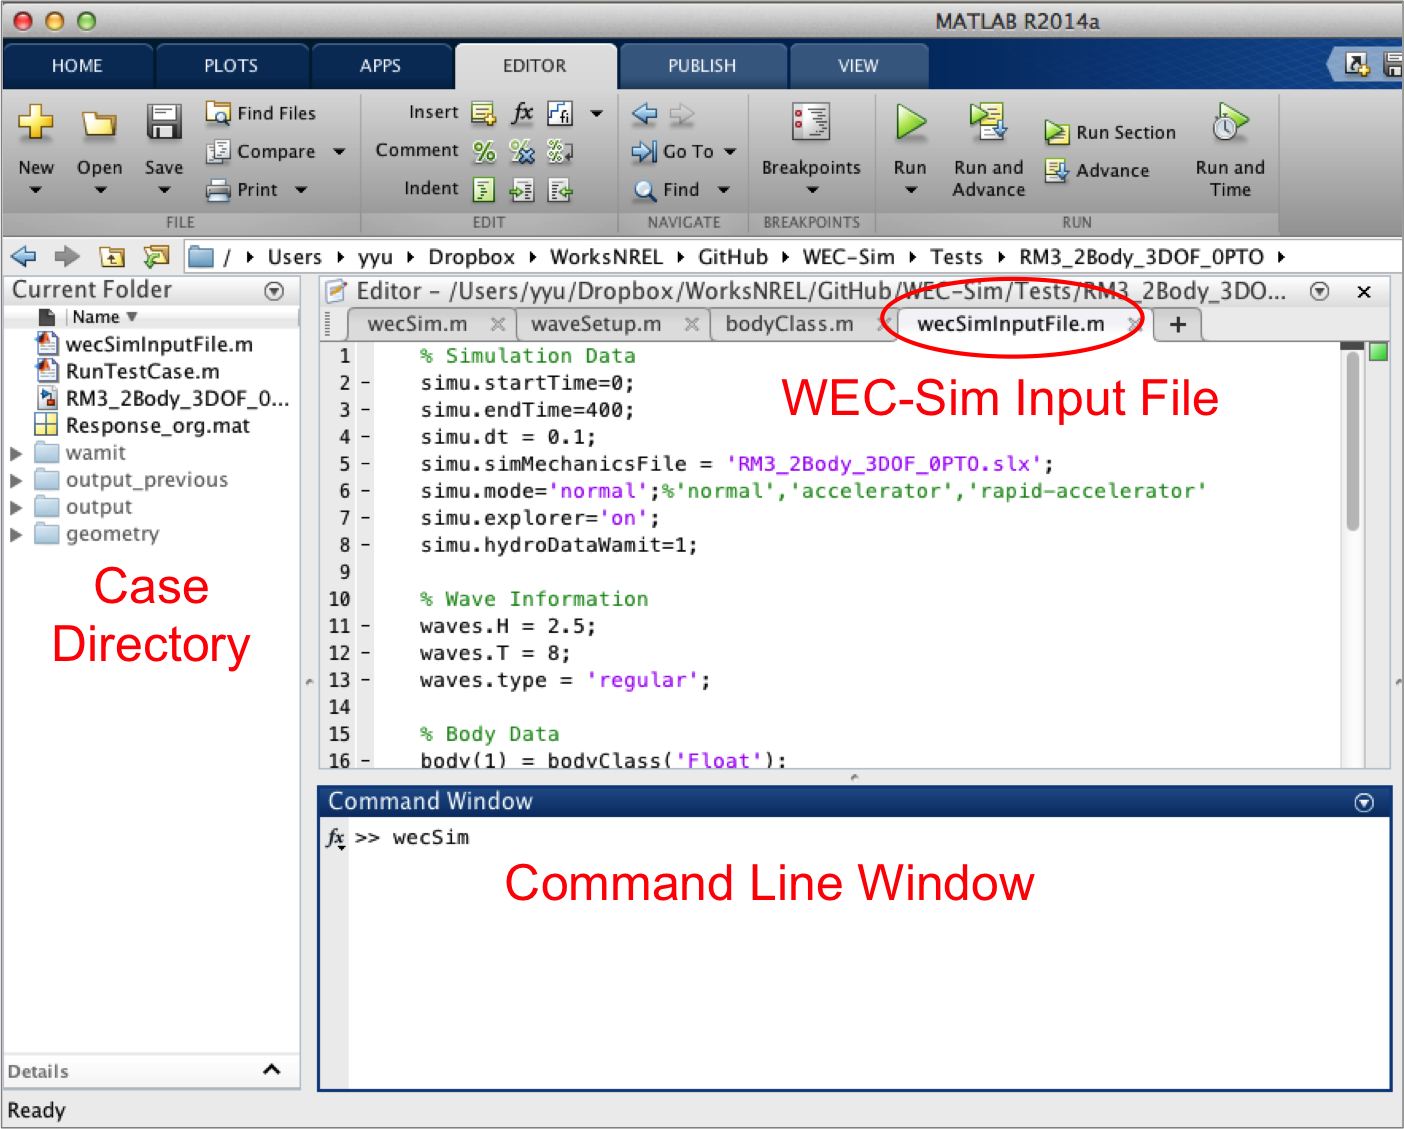
\includegraphics[scale=0.55]{gettingStarted/Figures/runWECSim_mod}\protect\caption{An example of running WEC-Sim}
\label{fig:exampleRunWECSim}
\end{figure}

\subsection{Simulation Outputs}\label{sec:simulationOutputs}
All simulation outputs are saved in the \texttt{output} variable within the MATLAB workspace. Specifically, the output variable contains forces and motions of the WEC bodies, PTSs, and constraints. The \texttt{output} data file also contains time step information from the simulation.

At the completion of a simulation, WEC-Sim also saves all simulation data in the \texttt{output} directory within the WEC-Sim case file in three data files:
\begin{description}
\item[\texttt{<case name>\_simulationLog.txt}]: This ascii text file contains all information displayed in the MATLAB command window during a simulation.
\item[\texttt{<caseName>\_output.mat}]: This MATLAB data file contains forces and motions of the WEC bodies, PTSs, and constraints. The data file also contains time step information from the simulation.
\item[\texttt{<caseName>\_matlabWorkspace}]: This MATLAB data file contains all workspace variables from the simulation. Note that this variable also contains the \texttt{output.mat} data in a variable named \texttt{output}.
\end{description}

\subsection{Postprocessing using User Defined Functions (UDFs)}
Just before completion of a simulation, WEC-Sim looks for a MATLAB m-file named \texttt{userDefinedFunctions.m} within the WEC-Sim case directory. If the file exist, and WEC-Sim executes any commands within this m-file. The user can add code to this m-file to perform common post-processing tasks before the simulation exits. One example would be to plot the device motions and forces acting on the bodies and joints of a WEC device. The RM3 test case provides an example of how to plot force and response using user defined functions. Note that the user can perform any calculation desired within the \texttt{userDefinedFunctions.m}, and the user has access to all data within the MATLAB workspace.
